\documentclass[12]{beamer}

\usetheme{Warsaw}
\usecolortheme{seahorse}%{lily} 
% \setbeamercolor{frametitle}{bg=blue,fg=yellow} 
%\beamersetaveragebackground{blue!10} 

\colorlet{mystruct}{structure} % Zapis struktury
\colorlet{structure}{magenta} % Nowa struktura
\definecolor{kolor1}{RGB}{255,255,255}
\definecolor{kolor2}{RGB}{0,51,154}
\setbeamercolor{structure}{fg=kolor2} %kolor struktury (wypunktowania, spis tresci itp)
\setbeamercolor{palette primary}{fg=kolor2,bg=kolor1} %kolor ”tego” z podrozdzialami i \frametitle{}
\setbeamercolor{palette quaternary}{fg=kolor1,bg=kolor2} %kolor ”tego” z rozdzialami
\setbeamercolor{normal text}{fg=black,bg=kolor1}
%normalny tekst i tlo
\setbeamercolor{titlelike}{parent=palette quaternary}
%kolory tytulu jak w palete quaternary
\setbeamercolor{block title}{fg=kolor1,bg=kolor2}
%tytul bloku, napis i tlo
\setbeamercolor{block body}{parent=palette primary,fg=black} %kolor ciala bloku

\usepackage[T1]{fontenc}
\usepackage[utf8]{inputenc}
\usepackage[english]{babel}

\usepackage{graphicx}
%\usepackage{array}
%\usepackage{amssymb}

\graphicspath{ {./images/} }


\title[Semantic Image Segmentation in Computer Vision]
{Semantic Image Segmentation in Computer Vision}

\author{Aneta Andrzejewska 200285 \and Michał Kącki 203206}
\date[EngThesisPresentation]{\today}

%\AtBeginSubsection[]
%{
%  \begin{frame}<beamer>{Outline
%    \tableofcontents[currentsection,currentsubsection]
%  \end{frame}
%}

\begin{document}

\begin{frame}
  \titlepage
\end{frame}

%\begin{frame}{Outline}
%  \tableofcontents
%  % You might wish to add the option [pausesections]
%\end{frame}


\section{Semantic Image Segmentation}

\subsection{Introduction}

\begin{frame}{Semantic Image Segmentation}

\begin{figure}
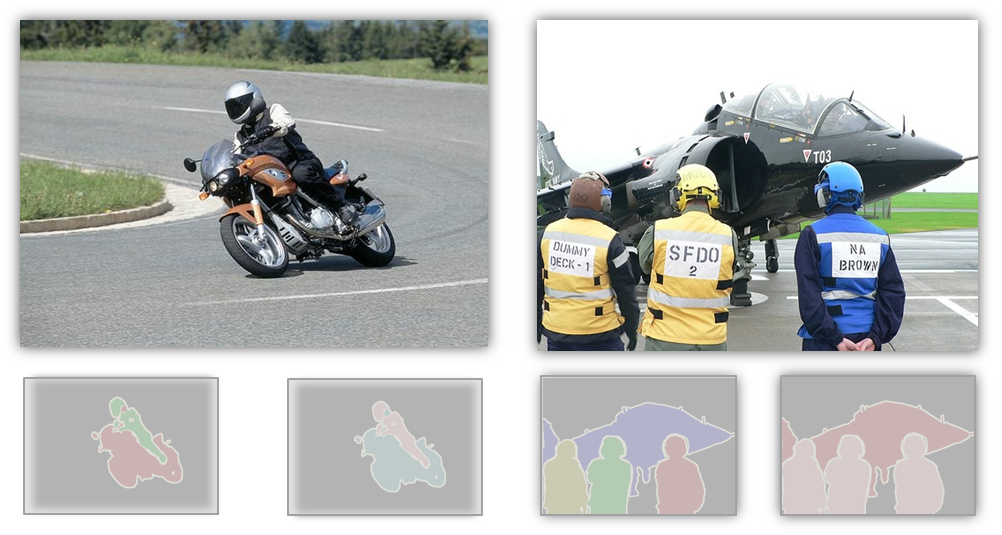
\includegraphics[width=\textwidth]{segmentation}
\end{figure}

\end{frame}

\begin{frame}{Object Segmentation}

\begin{figure}
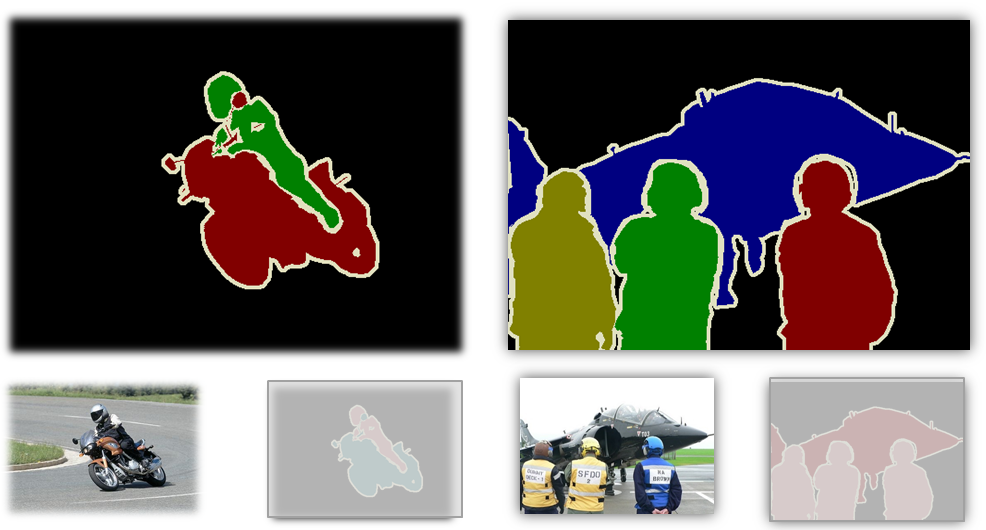
\includegraphics[width=\textwidth]{segmentation_object}
\end{figure}

\end{frame}

\begin{frame}{Class Segmentation}

\begin{figure}
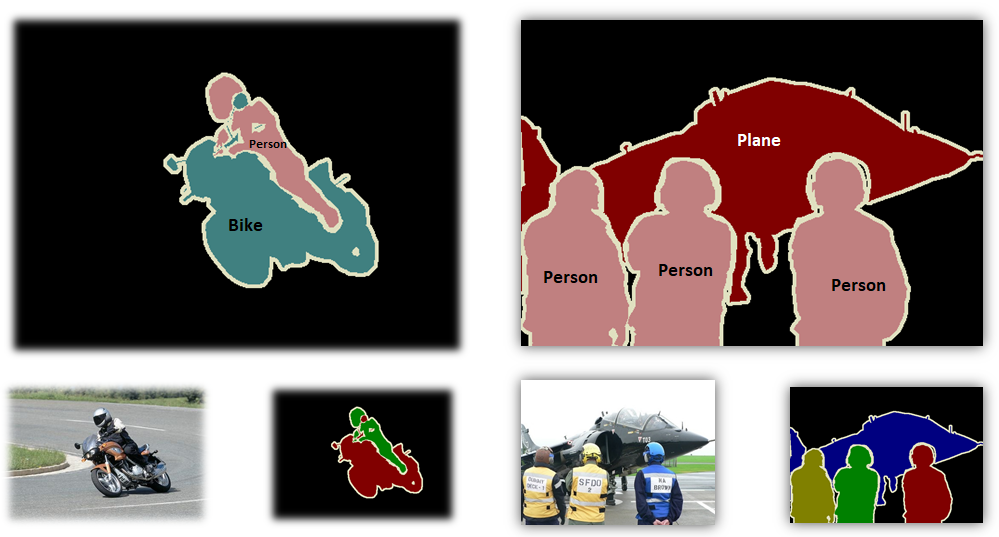
\includegraphics[width=\textwidth]{segmentation_class}
\end{figure}

\end{frame}

\begin{frame}{Semantic Segmentation goal}

\begin{figure}
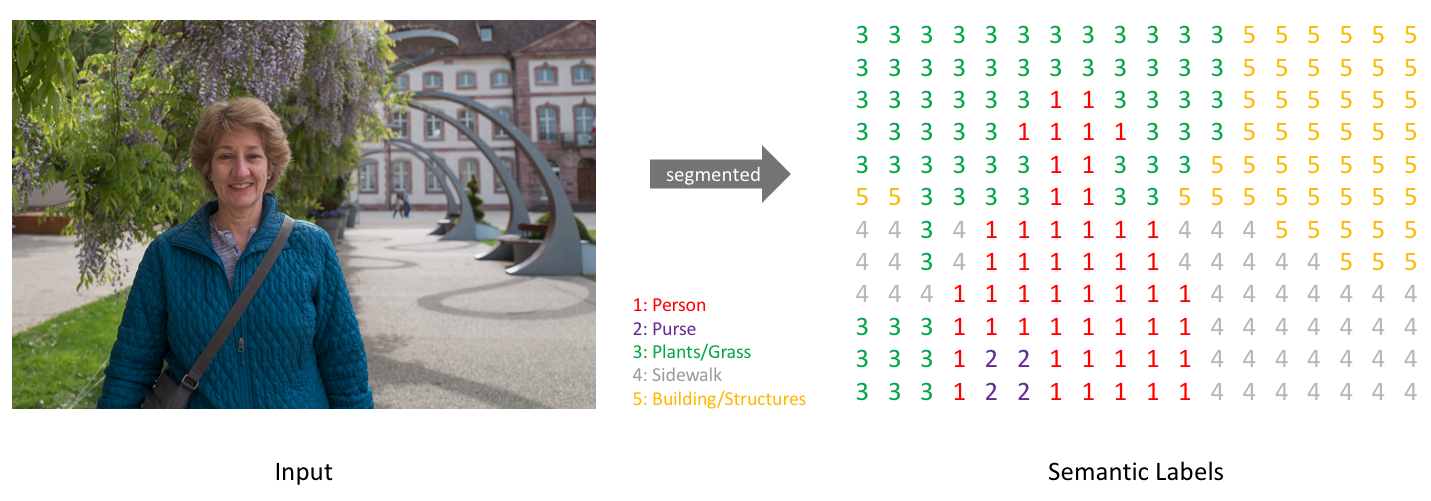
\includegraphics[width=\textwidth]{goal}
\end{figure}

\begin{itemize}
	\item Each pixel of an image is labelled with a corresponding class 
	\item No distinction between instances of the same class
\end{itemize}

\end{frame}



\subsection{Applications}

\begin{frame}{Pathological changes detection}

\begin{figure}
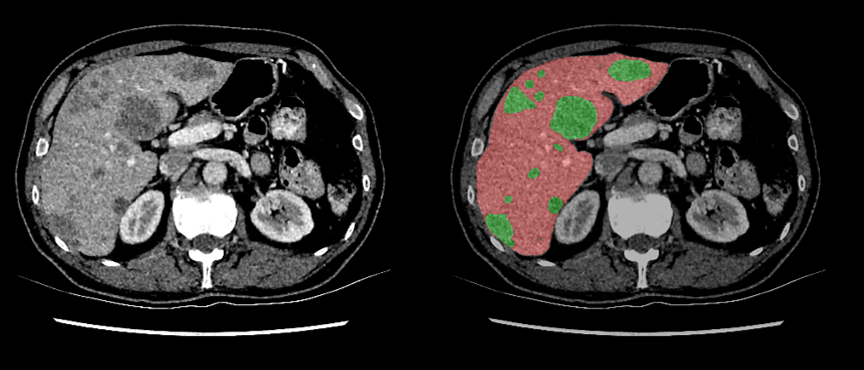
\includegraphics[width=\textwidth]{applications_medicine}
\end{figure}

\end{frame}

\begin{frame}{Autonomous driving}

\begin{figure}
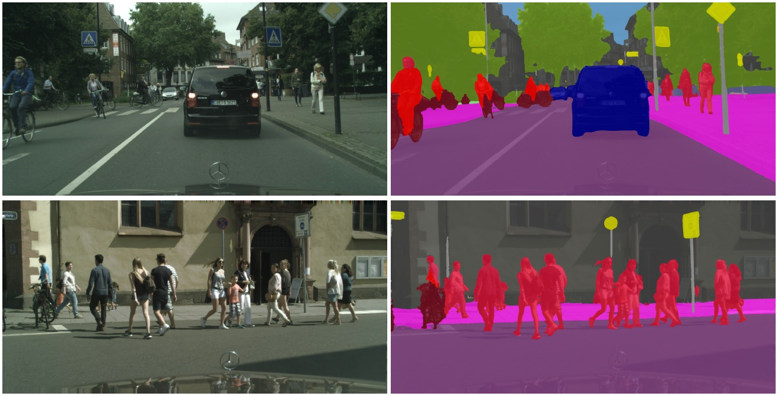
\includegraphics[width=\textwidth]{applications_driving}
\end{figure}

\end{frame}

\begin{frame}{Augmented reality}

\begin{figure}
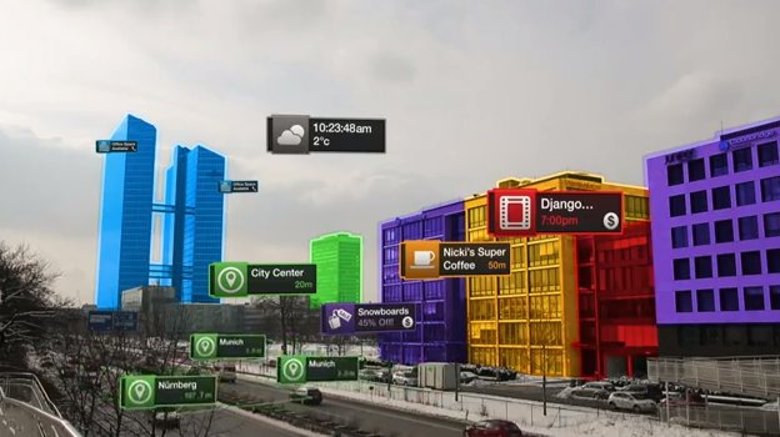
\includegraphics[width=\textwidth]{applications_vr}
\end{figure}

\end{frame}

\subsection{Segmentation methods}



\end{document}

